\documentclass{standalone}
\usepackage{tikz}
\usetikzlibrary{patterns, positioning}

\begin{document}
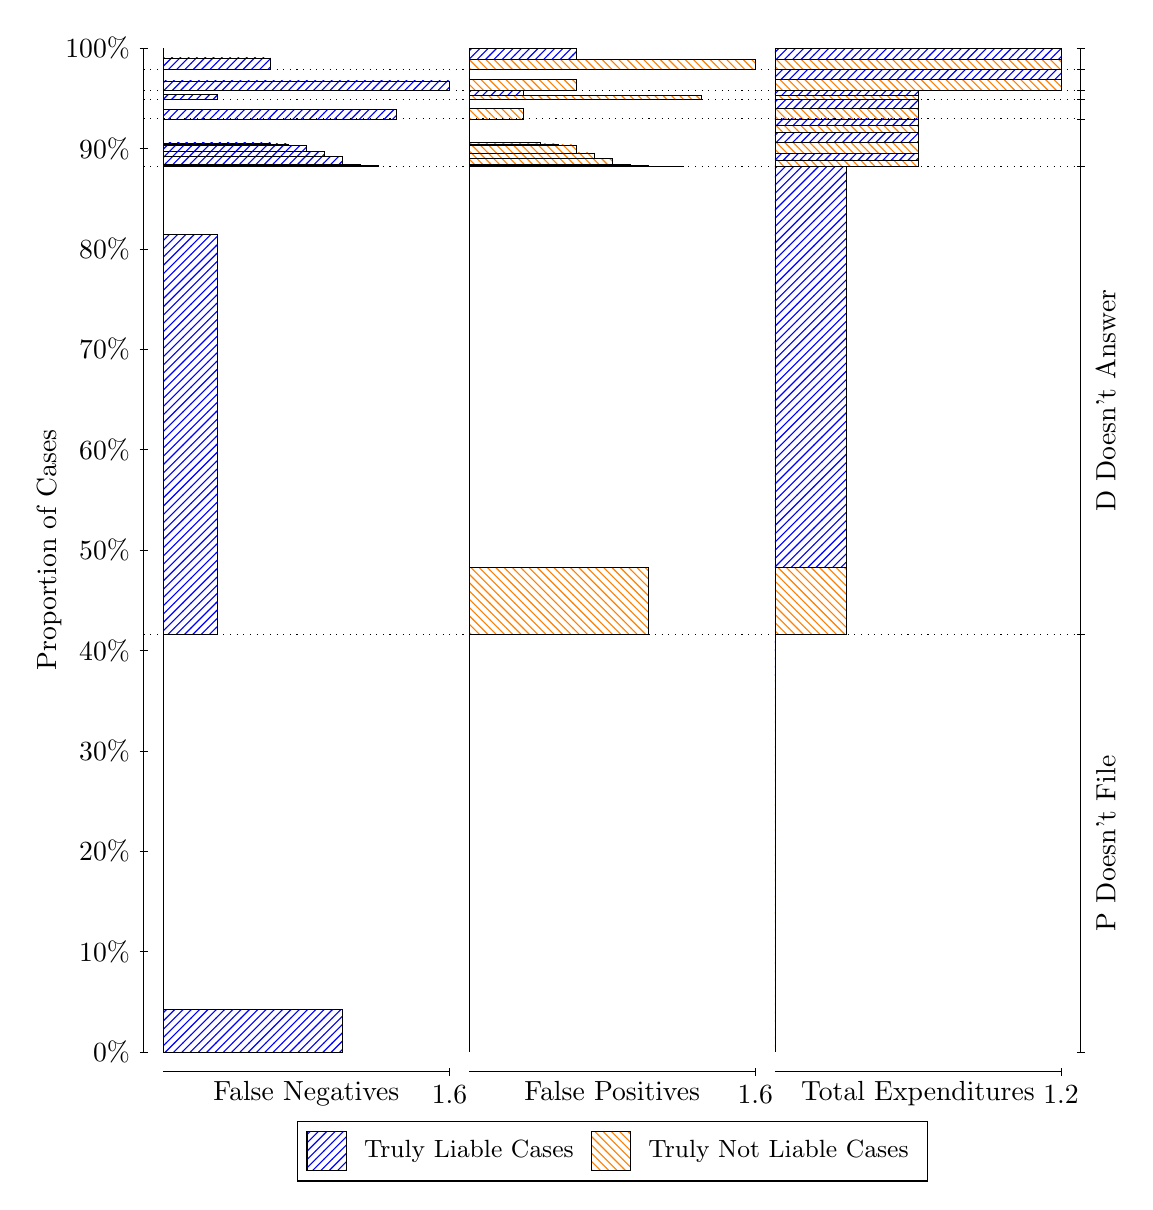
\begin{tikzpicture}
\draw[black, very thin] (1.5,1.75) -- (1.5,14.5);
\node[rotate=90, anchor=center] at (0.3, 8.125) {Proportion of Cases};
\draw[black, very thin] (1.45,1.75) -- (1.55,1.75);
\node[anchor=east] at (1.45, 1.75) {0\%};
\draw[black, very thin] (1.45,3.025) -- (1.55,3.025);
\node[anchor=east] at (1.45, 3.025) {10\%};
\draw[black, very thin] (1.45,4.3) -- (1.55,4.3);
\node[anchor=east] at (1.45, 4.3) {20\%};
\draw[black, very thin] (1.45,5.575) -- (1.55,5.575);
\node[anchor=east] at (1.45, 5.575) {30\%};
\draw[black, very thin] (1.45,6.85) -- (1.55,6.85);
\node[anchor=east] at (1.45, 6.85) {40\%};
\draw[black, very thin] (1.45,8.125) -- (1.55,8.125);
\node[anchor=east] at (1.45, 8.125) {50\%};
\draw[black, very thin] (1.45,9.4) -- (1.55,9.4);
\node[anchor=east] at (1.45, 9.4) {60\%};
\draw[black, very thin] (1.45,10.675) -- (1.55,10.675);
\node[anchor=east] at (1.45, 10.675) {70\%};
\draw[black, very thin] (1.45,11.95) -- (1.55,11.95);
\node[anchor=east] at (1.45, 11.95) {80\%};
\draw[black, very thin] (1.45,13.225) -- (1.55,13.225);
\node[anchor=east] at (1.45, 13.225) {90\%};
\draw[black, very thin] (1.45,14.5) -- (1.55,14.5);
\node[anchor=east] at (1.45, 14.5) {100\%};

\draw[black, very thin] (13.4,1.75) -- (13.4,14.5);
\draw[black, very thin] (13.35,1.75) -- (13.45,1.75);
\node[anchor=west] at (13.35, 1.75) {};
\draw[black, very thin] (13.35,7.0516) -- (13.45,7.0516);
\node[anchor=west] at (13.35, 7.0516) {};
\draw[black, very thin] (13.35,12.993) -- (13.45,12.993);
\node[anchor=west] at (13.35, 12.993) {};
\draw[black, very thin] (13.35,13.601) -- (13.45,13.601);
\node[anchor=west] at (13.35, 13.601) {};
\draw[black, very thin] (13.35,13.85) -- (13.45,13.85);
\node[anchor=west] at (13.35, 13.85) {};
\draw[black, very thin] (13.35,13.959) -- (13.45,13.959);
\node[anchor=west] at (13.35, 13.959) {};
\draw[black, very thin] (13.35,14.232) -- (13.45,14.232);
\node[anchor=west] at (13.35, 14.232) {};
\draw[black, very thin] (13.35,14.5) -- (13.45,14.5);
\node[anchor=west] at (13.35, 14.5) {};

\draw[black, very thin, pattern color=blue, pattern=north east lines] (1.75,1.75) rectangle (4.0208,2.2912);
\draw[black, very thin, pattern color=orange, pattern=north west lines] (1.75,2.2912) rectangle (1.75,7.0516);
\draw[black, very thin, pattern color=blue, pattern=north east lines] (1.75,7.0516) rectangle (2.4312,12.137);
\draw[black, very thin, pattern color=orange, pattern=north west lines] (1.75,12.137) rectangle (1.75,12.993);
\draw[black, very thin, pattern color=blue, pattern=north east lines] (1.75,12.993) rectangle (4.475,13.005);
\draw[black, very thin, pattern color=blue, pattern=north east lines] (1.75,13.005) rectangle (4.2479,13.019);
\draw[black, very thin, pattern color=blue, pattern=north east lines] (1.75,13.019) rectangle (4.0208,13.12);
\draw[black, very thin, pattern color=blue, pattern=north east lines] (1.75,13.12) rectangle (3.7937,13.124);
\draw[black, very thin, pattern color=blue, pattern=north east lines] (1.75,13.124) rectangle (3.7937,13.19);
\draw[black, very thin, pattern color=blue, pattern=north east lines] (1.75,13.19) rectangle (3.5667,13.263);
\draw[black, very thin, pattern color=blue, pattern=north east lines] (1.75,13.263) rectangle (3.3396,13.282);
\draw[black, very thin, pattern color=blue, pattern=north east lines] (1.75,13.282) rectangle (3.1125,13.294);
\draw[black, very thin, pattern color=blue, pattern=north east lines] (1.75,13.294) rectangle (2.8854,13.295);
\draw[black, very thin, pattern color=blue, pattern=north east lines] (1.75,13.295) rectangle (2.6583,13.296);
\draw[black, very thin, pattern color=orange, pattern=north west lines] (1.75,13.296) rectangle (1.75,13.601);
\draw[black, very thin, pattern color=blue, pattern=north east lines] (1.75,13.601) rectangle (4.7021,13.72);
\draw[black, very thin, pattern color=orange, pattern=north west lines] (1.75,13.72) rectangle (1.75,13.85);
\draw[black, very thin, pattern color=blue, pattern=north east lines] (1.75,13.85) rectangle (2.4312,13.907);
\draw[black, very thin, pattern color=orange, pattern=north west lines] (1.75,13.907) rectangle (1.75,13.959);
\draw[black, very thin, pattern color=blue, pattern=north east lines] (1.75,13.959) rectangle (5.3833,14.084);
\draw[black, very thin, pattern color=orange, pattern=north west lines] (1.75,14.084) rectangle (1.75,14.232);
\draw[black, very thin, pattern color=blue, pattern=north east lines] (1.75,14.232) rectangle (3.1125,14.375);
\draw[black, very thin, pattern color=orange, pattern=north west lines] (1.75,14.375) rectangle (1.75,14.5);
\draw[black, very thin, pattern color=orange, pattern=north west lines] (5.6333,1.75) rectangle (5.6333,6.5104);
\draw[black, very thin, pattern color=blue, pattern=north east lines] (5.6333,6.5104) rectangle (5.6333,7.0516);
\draw[black, very thin, pattern color=orange, pattern=north west lines] (5.6333,7.0516) rectangle (7.9042,7.9071);
\draw[black, very thin, pattern color=blue, pattern=north east lines] (5.6333,7.9071) rectangle (5.6333,12.993);
\draw[black, very thin, pattern color=orange, pattern=north west lines] (5.6333,12.993) rectangle (8.3583,12.994);
\draw[black, very thin, pattern color=orange, pattern=north west lines] (5.6333,12.994) rectangle (8.1313,12.995);
\draw[black, very thin, pattern color=orange, pattern=north west lines] (5.6333,12.995) rectangle (7.9042,13.007);
\draw[black, very thin, pattern color=orange, pattern=north west lines] (5.6333,13.007) rectangle (7.6771,13.026);
\draw[black, very thin, pattern color=orange, pattern=north west lines] (5.6333,13.026) rectangle (7.45,13.099);
\draw[black, very thin, pattern color=orange, pattern=north west lines] (5.6333,13.099) rectangle (7.2229,13.168);
\draw[black, very thin, pattern color=orange, pattern=north west lines] (5.6333,13.168) rectangle (6.9958,13.27);
\draw[black, very thin, pattern color=orange, pattern=north west lines] (5.6333,13.27) rectangle (6.7687,13.284);
\draw[black, very thin, pattern color=orange, pattern=north west lines] (5.6333,13.284) rectangle (6.5417,13.298);
\draw[black, very thin, pattern color=blue, pattern=north east lines] (5.6333,13.298) rectangle (6.0875,13.299);
\draw[black, very thin, pattern color=blue, pattern=north east lines] (5.6333,13.299) rectangle (5.8604,13.3);
\draw[black, very thin, pattern color=blue, pattern=north east lines] (5.6333,13.3) rectangle (5.6333,13.601);
\draw[black, very thin, pattern color=orange, pattern=north west lines] (5.6333,13.601) rectangle (6.3146,13.731);
\draw[black, very thin, pattern color=blue, pattern=north east lines] (5.6333,13.731) rectangle (5.6333,13.85);
\draw[black, very thin, pattern color=orange, pattern=north west lines] (5.6333,13.85) rectangle (8.5854,13.902);
\draw[black, very thin, pattern color=blue, pattern=north east lines] (5.6333,13.902) rectangle (6.3146,13.959);
\draw[black, very thin, pattern color=orange, pattern=north west lines] (5.6333,13.959) rectangle (6.9958,14.106);
\draw[black, very thin, pattern color=blue, pattern=north east lines] (5.6333,14.106) rectangle (5.6333,14.232);
\draw[black, very thin, pattern color=orange, pattern=north west lines] (5.6333,14.232) rectangle (9.2667,14.356);
\draw[black, very thin, pattern color=blue, pattern=north east lines] (5.6333,14.356) rectangle (6.9958,14.5);
\draw[black, very thin, pattern color=orange, pattern=north west lines] (9.5167,1.75) rectangle (9.5167,6.5104);
\draw[black, very thin, pattern color=blue, pattern=north east lines] (9.5167,6.5104) rectangle (9.5167,7.0516);
\draw[black, very thin, pattern color=orange, pattern=north west lines] (9.5167,7.0516) rectangle (10.425,7.9071);
\draw[black, very thin, pattern color=blue, pattern=north east lines] (9.5167,7.9071) rectangle (10.425,12.993);
\draw[black, very thin, pattern color=orange, pattern=north west lines] (9.5167,12.993) rectangle (11.333,13.079);
\draw[black, very thin, pattern color=blue, pattern=north east lines] (9.5167,13.079) rectangle (11.333,13.165);
\draw[black, very thin, pattern color=orange, pattern=north west lines] (9.5167,13.165) rectangle (11.333,13.299);
\draw[black, very thin, pattern color=blue, pattern=north east lines] (9.5167,13.299) rectangle (11.333,13.43);
\draw[black, very thin, pattern color=orange, pattern=north west lines] (9.5167,13.43) rectangle (11.333,13.515);
\draw[black, very thin, pattern color=blue, pattern=north east lines] (9.5167,13.515) rectangle (11.333,13.601);
\draw[black, very thin, pattern color=orange, pattern=north west lines] (9.5167,13.601) rectangle (11.333,13.731);
\draw[black, very thin, pattern color=blue, pattern=north east lines] (9.5167,13.731) rectangle (11.333,13.85);
\draw[black, very thin, pattern color=orange, pattern=north west lines] (9.5167,13.85) rectangle (11.333,13.902);
\draw[black, very thin, pattern color=blue, pattern=north east lines] (9.5167,13.902) rectangle (11.333,13.959);
\draw[black, very thin, pattern color=orange, pattern=north west lines] (9.5167,13.959) rectangle (13.15,14.106);
\draw[black, very thin, pattern color=blue, pattern=north east lines] (9.5167,14.106) rectangle (13.15,14.232);
\draw[black, very thin, pattern color=orange, pattern=north west lines] (9.5167,14.232) rectangle (13.15,14.356);
\draw[black, very thin, pattern color=blue, pattern=north east lines] (9.5167,14.356) rectangle (13.15,14.5);
\draw[black, dotted] (1.5,7.0516) -- (13.4,7.0516);
\draw[black, dotted] (1.5,12.993) -- (13.4,12.993);
\draw[black, dotted] (1.5,13.601) -- (13.4,13.601);
\draw[black, dotted] (1.5,13.85) -- (13.4,13.85);
\draw[black, dotted] (1.5,13.959) -- (13.4,13.959);
\draw[black, dotted] (1.5,14.232) -- (13.4,14.232);
\draw[black, very thin] (1.75,1.5) -- (5.3833,1.5);
\node[anchor=north] at (3.5667, 1.5) {False Negatives};
\draw[black, very thin] (5.3833,1.45) -- (5.3833,1.55);
\node[anchor=north] at (5.3833, 1.45) {1.6};

\draw[black, very thin] (5.6333,1.5) -- (9.2667,1.5);
\node[anchor=north] at (7.45, 1.5) {False Positives};
\draw[black, very thin] (9.2667,1.45) -- (9.2667,1.55);
\node[anchor=north] at (9.2667, 1.45) {1.6};

\draw[black, very thin] (9.5167,1.5) -- (13.15,1.5);
\node[anchor=north] at (11.333, 1.5) {Total Expenditures};
\draw[black, very thin] (13.15,1.45) -- (13.15,1.55);
\node[anchor=north] at (13.15, 1.45) {1.2};

\node[black, centered, rotate=90] at (13.72, 4.4008) {P Doesn't File};
\node[black, centered, rotate=90] at (13.72, 10.022) {D Doesn't Answer};






\draw (7.449999999999999,1.5) node[draw=none] (baseCoordinate) {};
\begin{scope}[align=center]
        \matrix[scale=0.5, draw=black, below=0.5cm of baseCoordinate, nodes={draw}, column sep=0.1cm]{
            \node[rectangle, draw, minimum width=0.5cm, minimum height=0.5cm, pattern=north east lines, pattern color=blue] {}; &
            \node[draw=none, font=\small] (B) {Truly Liable Cases}; &
            \node[rectangle, draw, minimum width=0.5cm, minimum height=0.5cm, pattern=north west lines, pattern color=orange] {}; &
            \node[draw=none, font=\small] (B) {Truly Not Liable Cases}; \\
            };
\end{scope}

\end{tikzpicture}
\end{document}